\documentclass[aspectratio=169]{beamer}

% BEAMER SETTINGS
\setbeamertemplate{navigation symbols}{}
\setbeamertemplate{enumerate items}[default]
\setbeamertemplate{footline}[frame number]

% CREATE SECTION SLIDES
\AtBeginSection[]{
  \begin{frame}
    \centering
    \Huge \insertsection
  \end{frame}
}

% PRESENTATION METADATA
\title{Comparing Models of Delta-Notch Signalling}
\author{Edwin Huras, Riley Wheadon, Ziyi Zhuang}
\institute{University of British Columbia}
\date{April 9, 2025}

\begin{document}

\begin{frame}
\titlepage
\end{frame}

% SECTION 1: RILEY (10m)
\section{Introduction}

\begin{frame}
  \frametitle{Introduction}
  % Pictures of organisms/systems that use delta notch signalling
\end{frame}

\begin{frame}
  \frametitle{The Signalling Pathway}
  % Diagram of Delta-Notch signalling pathway

  \begin{columns}

    \begin{column}{0.48\textwidth}
      
    \end{column}
      
    \begin{column}{0.48\textwidth}
      \begin{itemize}
        \item Ligands bind to a Notch receptor.
        \item This releases NICD in the cell.
        \item NICD promotes Notch, inhibits Delta, and promotes Serrate.
        \item \emph{Cis-inhibition} occurs between molecules from the same cell.
      \end{itemize}
    \end{column}
      
  \end{columns}

\end{frame}

\begin{frame}
  \frametitle{Previous Models}
  % Two columns -- compare Collier et al. to Boareto et al.
  \begin{columns}

      \onslide<1->{\begin{column}{0.48\textwidth}
        \textbf{Collier et al. (1996)}
        
        \begin{itemize}
          \item Is a deterministic ODE model.
          \item Not accurate to the biochemistry.
          \item Uses computational simulations.
          \item Looks at multiple 1D/2D domains.
        \end{itemize}
    \end{column}}
      
      \onslide<2->{\begin{column}{0.48\textwidth}
        \textbf{Boareto et al. (2015)}
        
        \begin{itemize}
          \item Is a deterministic ODE model.
          \item Accurate to the biochemistry.
          \item Uses bifurcation theory.
          \item Only analyzes two-cell domains.
        \end{itemize}
    \end{column}}
      
  \end{columns}
  \vspace{2em}

  \onslide<3->{We investigate how the results of these models change under the \textbf{Stochastic Differential Equation} (SDE) and \textbf{Agent-Based} formalisms.}

\end{frame}

\begin{frame}
  \frametitle{Our Assumptions}
  \begin{itemize}
    \item All ligands are Delta molecules (so we ignore Serrate).
    \item Delta molecules only bind to Notch receptors from neighbouring cells. 
    \item Reaction events follow a Poisson point process.
    \item Notch and Delta production are hill functions of NICD.
  \end{itemize}

\end{frame}

\begin{frame}

  \frametitle{Our Chemical Equations}

  \onslide<1->{Consider a cell $A$ with neighbour $B$. The Notch, Delta, and NICD concentrations of cell $A$ are given by $N_{A}$, $D_{A}$, and $I_{A}$ respectively (and similarly for cell $B$).
  
  \bigskip

  \begin{enumerate} 
    \item $N_{A} + D_{B} \rightarrow I_{A}$: Binding event. 
    \item $N_{A} \rightarrow \emptyset$: Notch decay.
    \item $D_{A} \rightarrow \emptyset$: Delta decay.
    \item $I_{A} \rightarrow \emptyset$: NICD decay.
    \item $\emptyset \rightarrow N_{A}$: Notch production.
    \item $\emptyset \rightarrow D_{A}$: Delta production.
\end{enumerate}}

  \bigskip

  \onslide<2->{In the \textbf{Agent-Based} model, we simulate these reactions directly using the \emph{Gillespie Algorithm}. Under our assumptions, this is the most accurate model.}

\end{frame}

\begin{frame}

  \frametitle{Differential Equation Models}

  \onslide<1->{In the \textbf{ODE} model, we approximate the reaction kinetics by simulating the agent-based model \emph{in expectation}. Since this model is deterministic, we ensure cell differentiation with an initial perturbation before all simulations.

$$\begin{aligned}
  \frac{dN}{dt} &= \frac{n_{m}I^2}{n_{0}^2 + I^2} - k_{T}ND_{ext} - \gamma N \\
  \frac{dD}{dt} &= \frac{d_{m}d_{0}^2}{d_{0}^2 + I^2} - k_{T}DN_{ext} - \gamma D \\
  \frac{dI}{dt} &= k_{T}ND_{ext} - \gamma_{I}I
\end{aligned}$$

  }

  \bigskip

  \onslide<2->{In the \textbf{SDE} model, we recreate some of the stochasticity of the agent-based model by adding an independent \emph{Wiener Process} to each equation above.}

\end{frame}

% SECTION 2: DORA (15m?)
\section{Derivation}
\begin{frame}{Preliminaries and Assumptions}
\begin{figure}
    \centering
    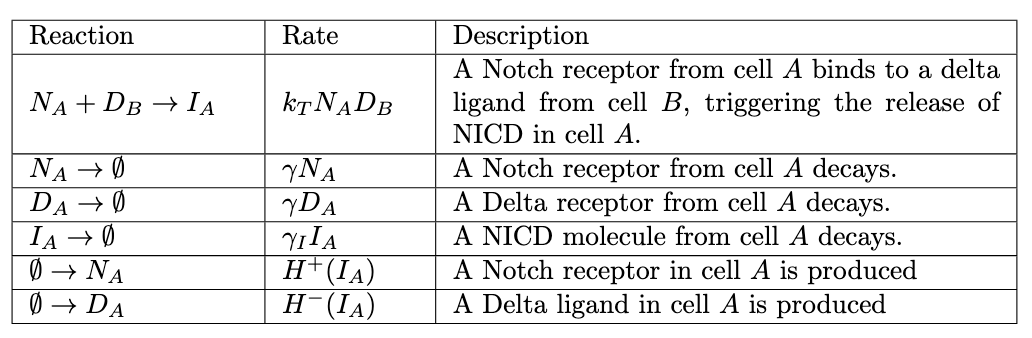
\includegraphics[width=0.9\linewidth]{image0.png}
\end{figure}
    Table 1: A list of possible reactions and their rates in a cell $A$ with neighbour $B$.
\end{frame}

\begin{frame}{Preliminaries and Assumptions}
Since there are $6$ possible reactions per cell, a system with $k$ cells will have $6k$ possible reactions to keep track of. \\
\hfill\break
In the following derivations, we focus on tracking a single cell (cell $A$) for simplicity.
\end{frame}

\begin{frame}{Derivation of Kolmogorov Forward Equation}
Let us define
\begin{itemize}
    \small \item $P(n,d,i,t)$: the probability of having $n$ Notch receptors, $d$ Delta ligands, and $i$ NICD molecules at time $t$.
    \small \item $D_{ext}$: the average Delta concentration over all neighbours of cell $A$.
\end{itemize}
The KFE describes how $P(n,d,i,t)$ changes over a small time step $\Delta t$:
\small \begin{align*}
P(n,d,i,t+\Delta t) &= P(n,d,i,t) \\
&+ P(n-1,d,i,t) \cdot H^+(i) \Delta t \quad \text{(Notch production)} \\
&+ P(n,d-1,i,t) \cdot H^-(i) \Delta t \quad \text{(Delta production)} \\
&+ P(n+1,d,i,t) \cdot \gamma(n+1)\Delta t \quad \text{(Notch decay)} \\
&+ P(n,d+1,i,t) \cdot \gamma(d+1)\Delta t \quad \text{(Delta decay)} \\
&+ P(n,d,i+1,t) \cdot \gamma_I(i+1)\Delta t \quad \text{(NICD decay)} \\
&+ P(n+1,d,i-1,t) \cdot k_T(n+1)D_{ext}\Delta t \quad \text{(Trans-activation)} \\
&- P(n,d,i,t) \cdot [H^+(i) + H^-(i) + \gamma n + \gamma d + \gamma_I i + k_T n D_{ext}]\Delta t
\end{align*}
\end{frame}

\begin{frame}{Derivation of Kolmogorov Forward Equation}
Rearranging to find the time derivative and taking the limit as $\Delta t \rightarrow 0$:

\begin{align*}
\frac{\partial P(n,d,i,t)}{\partial t} &= P(n-1,d,i,t) \cdot H^+(i) \\
&+ P(n,d-1,i,t) \cdot H^-(i) \\
&+ P(n+1,d,i,t) \cdot \gamma(n+1) \\
&+ P(n,d+1,i,t) \cdot \gamma(d+1) \\
&+ P(n,d,i+1,t) \cdot \gamma_I(i+1) \\
&+ P(n+1,d,i-1,t) \cdot k_T(n+1)D_{ext} \\
&- P(n,d,i,t) \cdot [H^+(i) + H^-(i) + \gamma n + \gamma d + \gamma_I i + k_T n D_{ext}]
\end{align*}

\end{frame}

\begin{frame}{Matrix Formulation}
The Kolmogorov forward equation can be expressed in matrix form as:
\[
\frac{d\vec{P}(t)}{dt} = \mathbf{A} \vec{P}(t)
\]

where $\vec{P}(t)$ is a column vector containing the probabilities for all possible states, and $\mathbf{A}$ is the transition rate matrix.\\
Each entry $A_{i,j}$ represents the transition rate from state $i$ to state $j$. The diagonal elements $A_{i,i}$ contain the negative sum of all outgoing rates from state $i$.

\end{frame}

\begin{frame}{Matrix Formulation}
Each state in our system is described by ($n$,$d$,$i$), but the matrix form needs a single index.
\vfill
\pause
We flatten the 3D state space into a 1D list.\\
\begin{itemize}
    \item We encode ($n$,$d$,$i$) into a single index — just like how multidimensional data (e.g., images, simulation grids) are stored in computer memory.
\end{itemize}
\end{frame}

\begin{frame}{Matrix Formulation}
To construct the matrix $\mathbf{A}$, we first establish a one-to-one mapping between the three-dimensional state space $(n,d,i)$ and a one-dimensional index $k$. \\~\\

We set $n_{max}$, $d_{max}$, and $i_{max}$ as large enough bounds for Notch, Delta, and NICD in cell $A$. These define the size of our 3D ``box" of possible states. \\
\textit{Remark:} These are not strict limits but chosen large enough to technically capture all relevant dynamics.
\end{frame}

\begin{frame}{Matrix Formulation}
For a system with ``maximum" values $n_{max}$, $d_{max}$, and $i_{max}$, we define:
\[
k(n,d,i) = n \cdot (d_{max}+1) \cdot (i_{max}+1) + d \cdot (i_{max}+1) + i
\]
for $0 \leq n \leq n_{max}, \; 0 \leq d \leq d_{max}, \; 0 \leq i \leq i_{max}$. \\
The inverse mapping gives:
\begin{align*}
n(k) &= \left\lfloor \frac{k}{(d_{max}+1) \cdot (i_{max}+1)} \right\rfloor \\
d(k) &= \left\lfloor \frac{k \bmod ((d_{max}+1) \cdot (i_{max}+1))}{i_{max}+1} \right\rfloor \\
i(k) &= k \bmod (i_{max}+1)
\end{align*}
\end{frame}

\begin{frame}{Matrix Formulation}
With this mapping, we can now define the elements of matrix $\mathbf{A}$. Let $k$ and $k'$ be the indices corresponding to states $(n,d,i)$ and $(n',d',i')$ respectively:

\begin{align*}
A_{k,k'} = 
\begin{cases}
H^+(i) & \text{if } (n',d',i') = (n+1,d,i) \quad \text{(Notch production)} \\
H^-(i) & \text{if } (n',d',i') = (n,d+1,i) \quad \text{(Delta production)} \\
\gamma(n) & \text{if } (n',d',i') = (n-1,d,i) \quad \text{(Notch decay)} \\
\gamma(d) & \text{if } (n',d',i') = (n,d-1,i) \quad \text{(Delta decay)} \\
\gamma_I(i) & \text{if } (n',d',i') = (n,d,i-1) \quad \text{(NICD decay)} \\
k_T(n)D_{ext} & \text{if } (n',d',i') = (n-1,d,i+1) \quad \text{(Trans-activation)} \\
-v & \text{if } k' = k \quad \text{(Diagonal terms)}
\end{cases}
\end{align*}
\end{frame}

\begin{frame}{Matrix Formulation}
Note that $A_{k,k'}$ represents the transition rate from state $k$ to state $k'$. The diagonal elements $A_{k,k}$ are the negative sum of all outgoing rates from state $k$:

\[
A_{k,k} = -v_k =-[H^+(i) + H^-(i) + \gamma n + \gamma d + \gamma_I i + k_T n D_{ext} + k_T d N_{ext}]
\]

where $(n,d,i)$ is the state corresponding to index $k$.\\
\textit{Recall:} We assume that reaction times follow a Poisson point process.\\~\\

\pause

The resulting matrix $\mathbf{A}$ is a sparse matrix with the following properties:
\begin{itemize}
    \item Dimension: $(n_{max}+1) \cdot (d_{max}+1) \cdot (i_{max}+1) \times (n_{max}+1) \cdot (d_{max}+1) \cdot (i_{max}+1)$
    \item Number of non-zero elements: $\approx 7 \cdot (n_{max}+1) \cdot (d_{max}+1) \cdot (i_{max}+1)$
\end{itemize}
\end{frame}

\begin{frame}{Matrix Formulation}
The corresponding transition matrix $\mathbf{A}$ would be:

\small \begin{align*}
\mathbf{A} = 
\begin{pmatrix}
-v_{000} & \alpha_{000,001} & \alpha_{000,010} & \alpha_{000,011} & \alpha_{000,100} & \alpha_{000,101} & \alpha_{000,110} & \alpha_{000,111} \\
\alpha_{001,000} & -v_{001} & \alpha_{001,010} & \alpha_{001,011} & \alpha_{001,100} & \alpha_{001,101} & \alpha_{001,110} & \alpha_{001,111} \\
\alpha_{010,000} & \alpha_{010,001} & -v_{010} & \alpha_{010,011} & \alpha_{010,100} & \alpha_{010,101} & \alpha_{010,110} & \alpha_{010,111} \\
\alpha_{011,000} & \alpha_{011,001} & \alpha_{011,010} & -v_{011} & \alpha_{011,100} & \alpha_{011,101} & \alpha_{011,110} & \alpha_{011,111} \\
\alpha_{100,000} & \alpha_{100,001} & \alpha_{100,010} & \alpha_{100,011} & -v_{100} & \alpha_{100,101} & \alpha_{100,110} & \alpha_{100,111} \\
\alpha_{101,000} & \alpha_{101,001} & \alpha_{101,010} & \alpha_{101,011} & \alpha_{101,100} & -v_{101} & \alpha_{101,110} & \alpha_{101,111} \\
\alpha_{110,000} & \alpha_{110,001} & \alpha_{110,010} & \alpha_{110,011} & \alpha_{110,100} & \alpha_{110,101} & -v_{110} & \alpha_{110,111} \\
\alpha_{111,000} & \alpha_{111,001} & \alpha_{111,010} & \alpha_{111,011} & \alpha_{111,100} & \alpha_{111,101} & \alpha_{111,110} & -v_{111}
\end{pmatrix}
\end{align*}

where:
\begin{align*}
\alpha_{ndi,n'd'i'} = 
\begin{cases}
H^+(i) + H^-(i) + \gamma n + \gamma d + \gamma_I i + k_T n D_{ext} + k_T d N_{ext} & \text{if } (n,d,i) \rightarrow (n',d',i') \\
0 & \text{otherwise}
\end{cases}
\end{align*}

\end{frame}

\begin{frame}{Remarks}
Let us consider

\begin{itemize}
    \item A one-cell system: $P(n,d,i,t+\Delta t)$ \\
    A $k$-cell system: $P(n_1,d_1,i_1,n_2,d_2,i_2,...,n_k,d_k,i_k,t+\Delta t)$\\
    \item $D_{ext}$ (the average Delta concentration over all neighbours of cell $A$)\\ can vary depending on the choice of domain.
\end{itemize}
\vfill
\pause
The complexity of a single cell highlights the need for numerical methods to model interactions between cells.
\end{frame}

% SECTION 3: EDWIN (20m?)
\section{Results}

\begin{frame}
  \frametitle{Comparing Two-Cell Models}
\end{frame}

\begin{frame}
  \frametitle{Noise in the SDE Model}
\end{frame}

\begin{frame}
  \frametitle{Stability Analysis}

  \onslide<1->{
    We tested model stability by perturbing $N_{m}$, $D_{m}$, $K_{T}$, $\gamma$, and $\gamma_{I}$.
$$\begin{aligned}
  \frac{dN}{dt} &= \frac{n_{m}I^2}{n_{0}^2 + I^2} - k_{T}ND_{ext} - \gamma N \\
  \frac{dD}{dt} &= \frac{d_{m}d_{0}^2}{d_{0}^2 + I^2} - k_{T}DN_{ext} - \gamma D \\
  \frac{dI}{dt} &= k_{T}ND_{ext} - \gamma_{I}I
\end{aligned}$$
  }

  \onslide<2->{
    Due to computational limitations, we investigated the $2$-dimensional subspaces of our $5$-dimensional parameter space using the following algorithm:
    \begin{itemize}
      \item Run the two-cell model on a $25 \times 25$ grid of points spanning $2$ OOMs.
      \item Take the convex hull of the points at which the cells differentiated.
    \end{itemize}
}

\end{frame}

\begin{frame}
  \frametitle{Stability Analysis Results}
\end{frame}

\begin{frame}
  \frametitle{Simulations on Linear Domains}
\end{frame}

\begin{frame}
  \frametitle{Patterns on Linear Domains}
\end{frame}

\begin{frame}
  \frametitle{Simulations on Hexagonal Domains}
\end{frame}

\begin{frame}
  \frametitle{Patterns on Hexagonal Domains}
\end{frame}

\section{End}

\end{document}
